% Author:Zhuming Shi, Peking University
% Theme from https://github.com/matze/mtheme

% \documentclass[12pt,AutoFakeBold,aspectratio=169,mathserif]{beamer}
\documentclass[AutoFakeBold]{beamer}
\usepackage[english]{babel}

\usetheme{metropolis}

\usepackage{fontspec}% 控制字体
% \setmainfont{Times New Roman}% 英文字体
\newfontfamily\arial{Arial}% Arial字体

\usepackage{xeCJK} % 中文支持
\setCJKmainfont{SimHei} % 中文字体
\XeTeXlinebreaklocale "zh"%中文自动换行
\XeTeXlinebreakskip = 0pt plus 1pt%中文自动换行

\usepackage{graphicx}
\usepackage{subfigure}
\usepackage{caption}

\usepackage{amsthm,amsmath,amssymb,mathrsfs}% 数学符号和花体支持
\usepackage{booktabs}% 绘制三线表
\usepackage{latexsym}% 绘制特殊数学符号
\usepackage{siunitx}% 数学模式中使用SI单位

\usepackage[version=3]{mhchem}% 化学反应式
\usepackage{epstopdf}% 插入ChemDraw的.eps结构图

% 代码环境
\usepackage{listings}
\usepackage{color}

\definecolor{dkgreen}{rgb}{0,0.6,0}
\definecolor{gray}{rgb}{0.5,0.5,0.5}
\definecolor{mauve}{rgb}{0.58,0,0.82}

\lstset{frame=tb,
  language=c++,
  aboveskip=3mm,
  belowskip=3mm,
  showstringspaces=false,
  columns=flexible,
  basicstyle={\small\ttfamily},
  numbers=none,
  numberstyle=\tiny\color{gray},
  keywordstyle=\color{blue},
  commentstyle=\color{dkgreen},
  stringstyle=\color{mauve},
  breaklines=true,
  breakatwhitespace=true,
  tabsize=3
}

\setbeamerfont{footnote}{size=\tiny}

\newcommand{\unknow}[1]{{\arial \textbf{#1}}}%未知化合物格式
\newcommand{\substance}[1]{\textbf{\emph{#1}}}%矿物名称格式

% \setbeamertemplate{background}{\includegraphics[height=\paperheight]{figures/sisters1080.png}}

\makeatletter 
\renewcommand{\@thesubfigure}{\hskip\subfiglabelskip}
\makeatother

\title{怎样做一个pre}
\author{第10组\quad 徐希彦\quad 张乐行\quad 施朱鸣}
\date{1月6日}

\begin{document}
    {
    % \setbeamertemplate{background}{\includegraphics[height=\paperheight]{figures/sisters1080.png}}
    % \setbeamertemplate{background}{
\includegraphics[height=\paperheight]{figures/misaka1080.jpg}}
    % \setbeamertemplate{background}{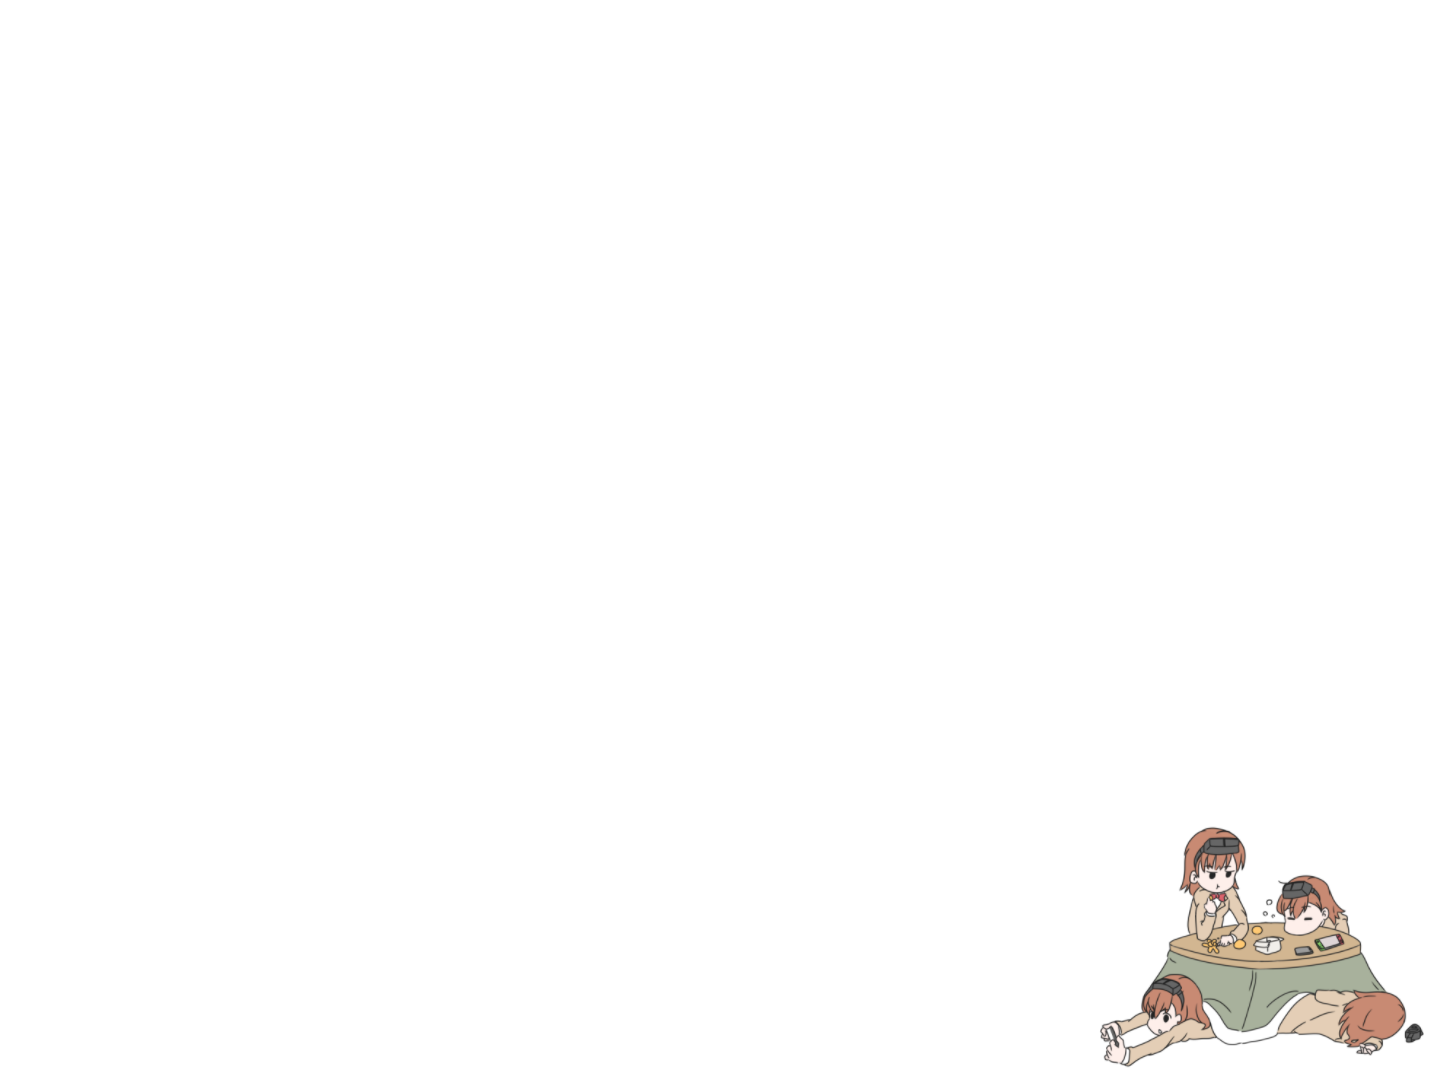
\includegraphics[height=\paperheight]{figures/misaka43.jpg}}
    
    \begin{frame}
    \titlepage
    \end{frame}
    \frame{\frametitle{Outline}\tableofcontents[hideallsubsections]}
    \section{面向对象}
    \begin{frame}
        \frametitle{面向对象}
    
        \begin{itemize}
            \item 如何让狒狒学会死锁(deadlock)?
        \end{itemize}
    
        \begin{figure}
            \centering
            \subfigure[]{
                
\includegraphics[height=.3\paperheight]{figures/1.jpg}
            }
            \subfigure[]{
                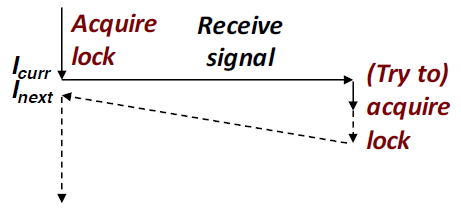
\includegraphics[height=.3\paperheight]{figures/2.png}
            }
        \end{figure}
    \end{frame}

    \begin{frame}
        \frametitle{面向对象}
    
        \begin{figure}
            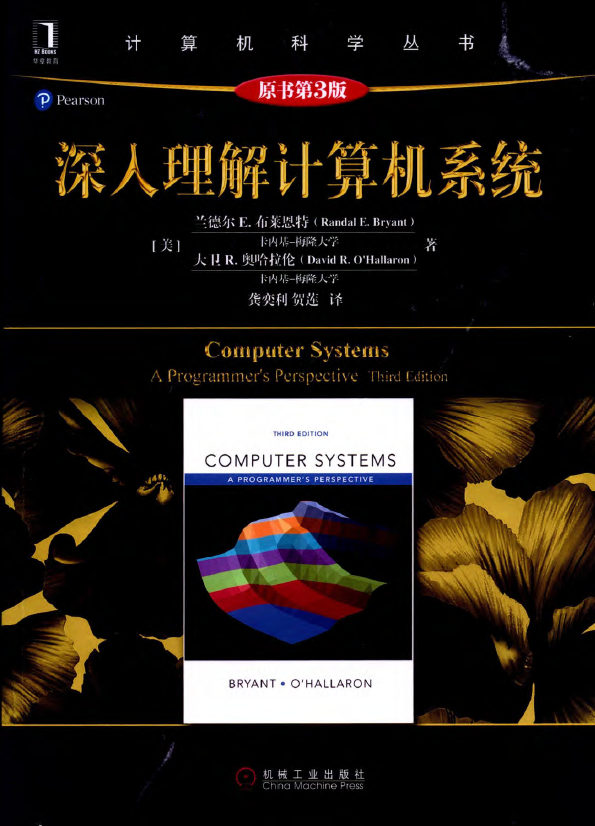
\includegraphics[height=.5\paperheight]{figures/3.png}
        \end{figure}
    
    \end{frame}

    \begin{frame}
        \frametitle{面向对象}
    
        \begin{figure}
            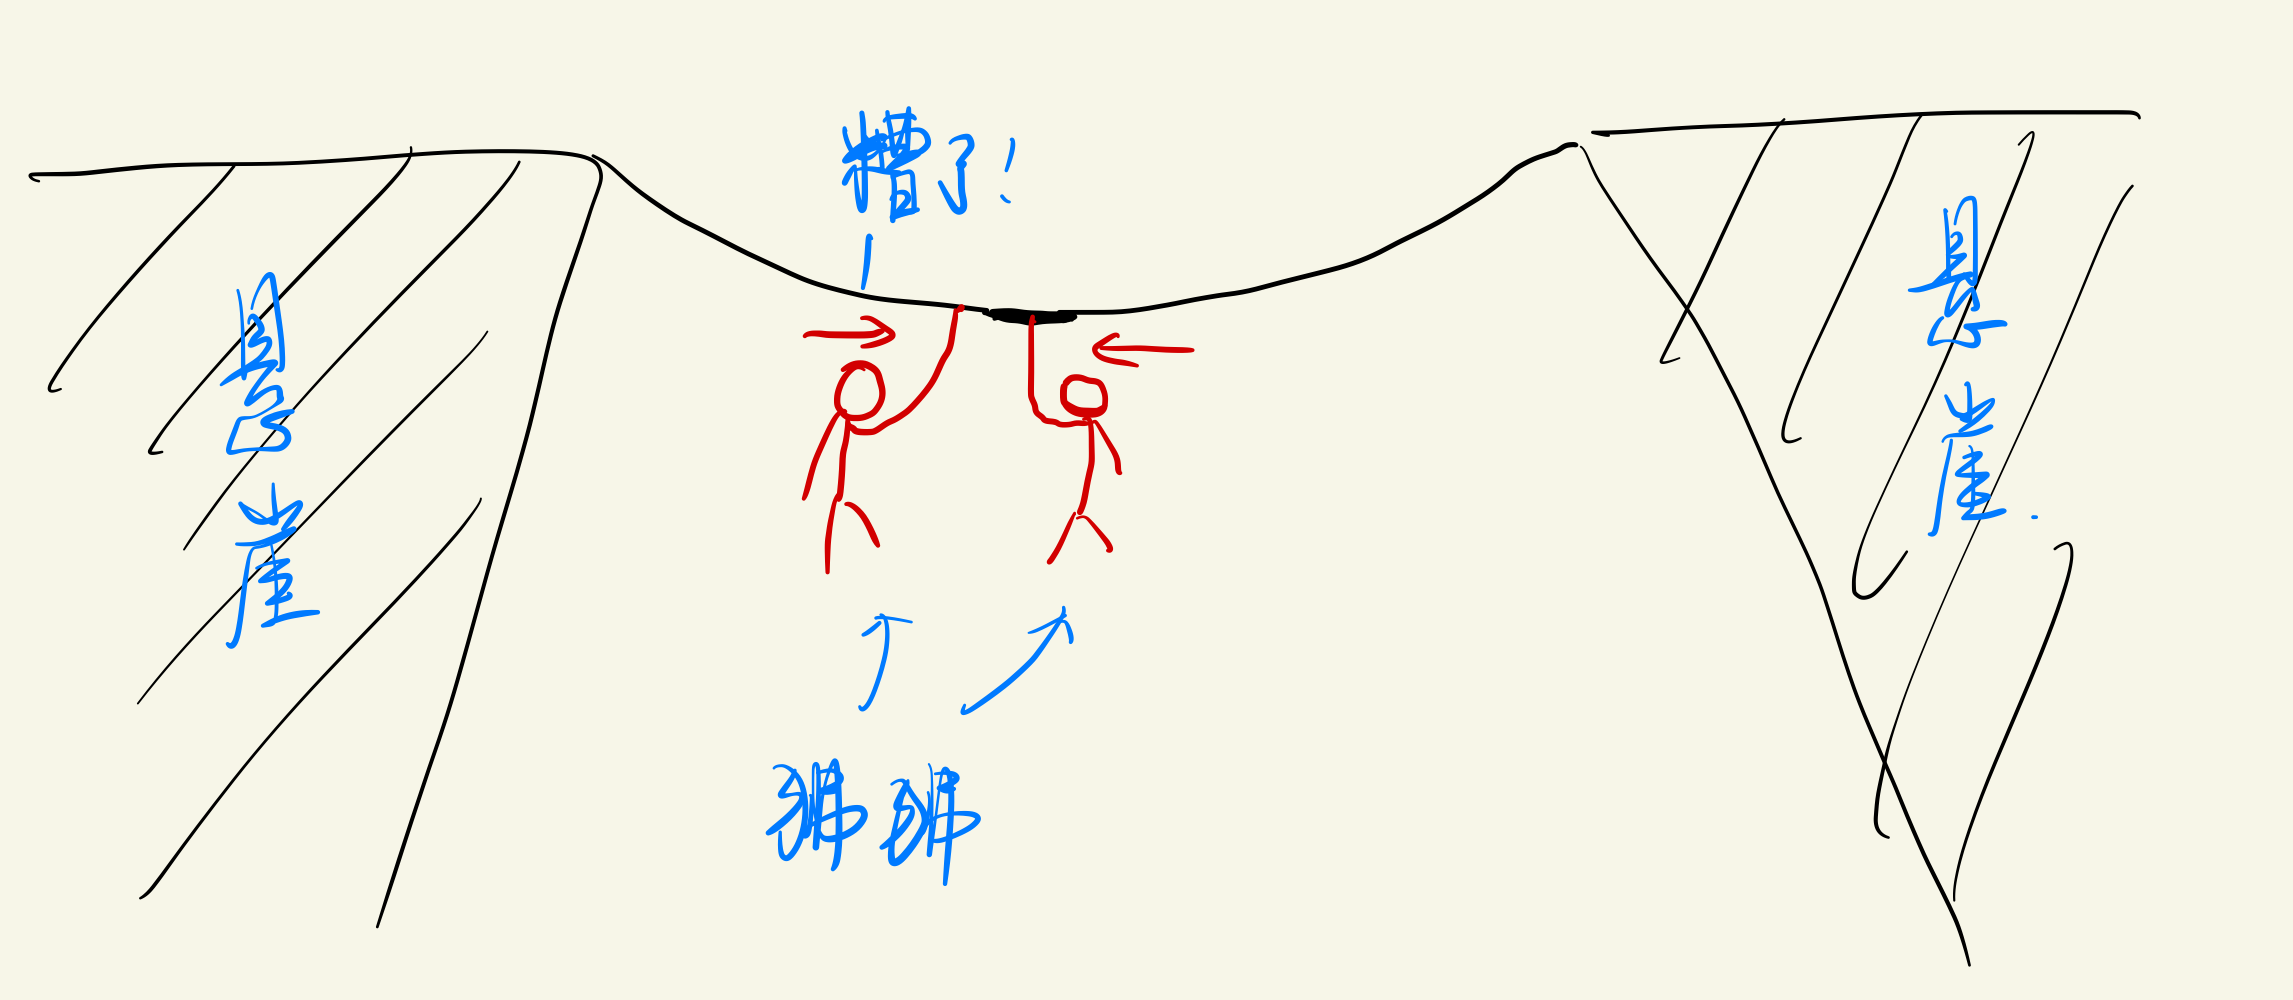
\includegraphics[height=.4\paperheight]{figures/4.png}
        \end{figure}
    
    \end{frame}

    \section{面向目的}

    \begin{frame}
        \frametitle{面向目的}
    
        \begin{itemize}
            \item 数分课?
            \item 轮转导师介绍?
        \end{itemize}
    
    \end{frame}

    \section{想清楚}

    \begin{frame}
        \frametitle{想清楚}
    
        \begin{itemize}
            \item 要做什么?
            \item 重点是什么?
            \item 想让听众思考些什么?
        \end{itemize}
    
    \end{frame}

    \section{说人话}

    \begin{frame}
        \frametitle{说人话}
    
        \begin{center}
            "数学分析,就是要我们把话说清楚"

                            ————谭小江老师
        \end{center}
    
    \end{frame}
    
    \begin{frame}
        \frametitle{说人话}
        \(E(X-Y)\geq \frac{n}{2k}\)是什么意思?它和最大独立子图有什么关系?
        \begin{figure}
            \subfigure[]{
                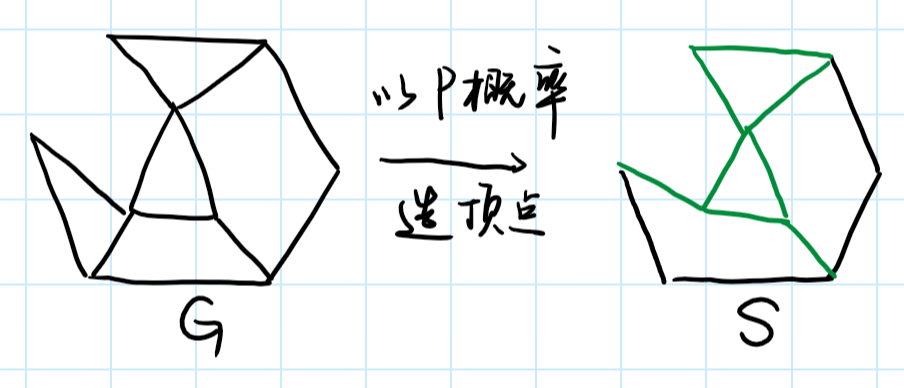
\includegraphics[width=.5\paperwidth]{figures/szm1.png}
            }
            \subfigure[]{
                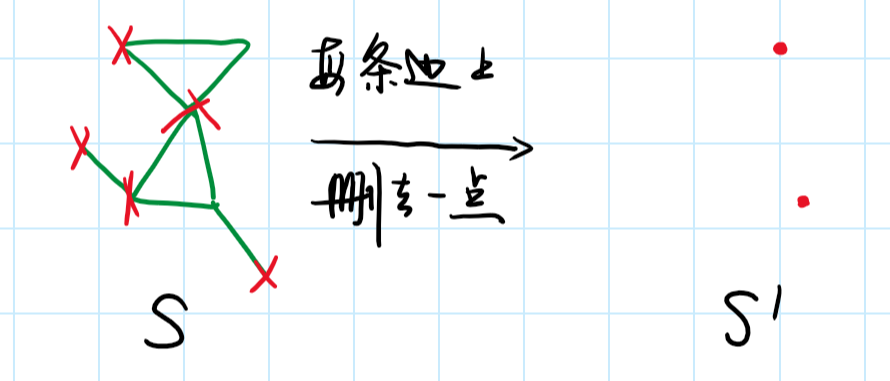
\includegraphics[width=.5\paperwidth]{figures/szm2.png}
            }
        \end{figure}
    
    \end{frame}
    
    \section{有亮点}

    \begin{frame}
        \frametitle{有亮点}
    
        
    
    \end{frame}

    \begin{frame}
        \frametitle{有亮点}
    
        没有亮点没有亮点没有亮点没有亮点没有亮点没有亮点没有亮点没有亮点

        \textbf{有亮点}:有亮点有亮点有亮点有亮点有亮点有亮点

        \begin{itemize}
            \item 亮点1:有亮点有亮点有亮点
            \item 亮点2:有亮点有亮点有亮点
        \end{itemize}
    
    \end{frame}

    \section{不要忘了图片}

    \begin{frame}
        \frametitle{不要忘了图片}
    
        \begin{figure}
            \subfigure[]{
                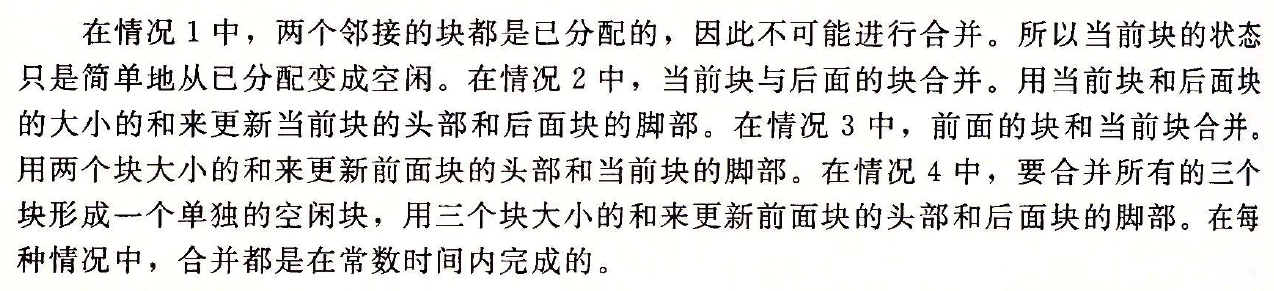
\includegraphics[width=.5\paperwidth]{figures/zlx1.png}
            }
            \subfigure[]{
                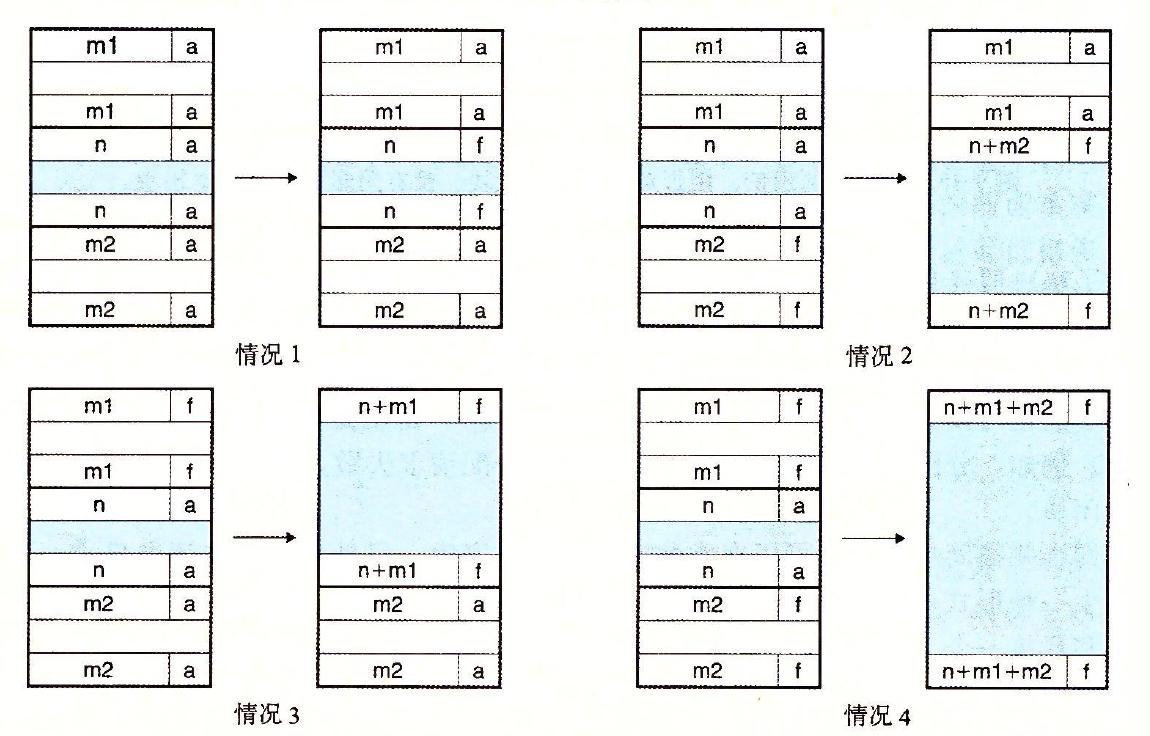
\includegraphics[width=.5\paperwidth]{figures/zlx2.png}
            }
        \end{figure}
    
    \end{frame}

    \begin{frame}
        \frametitle{不要忘了图片}
    
        \begin{figure}
            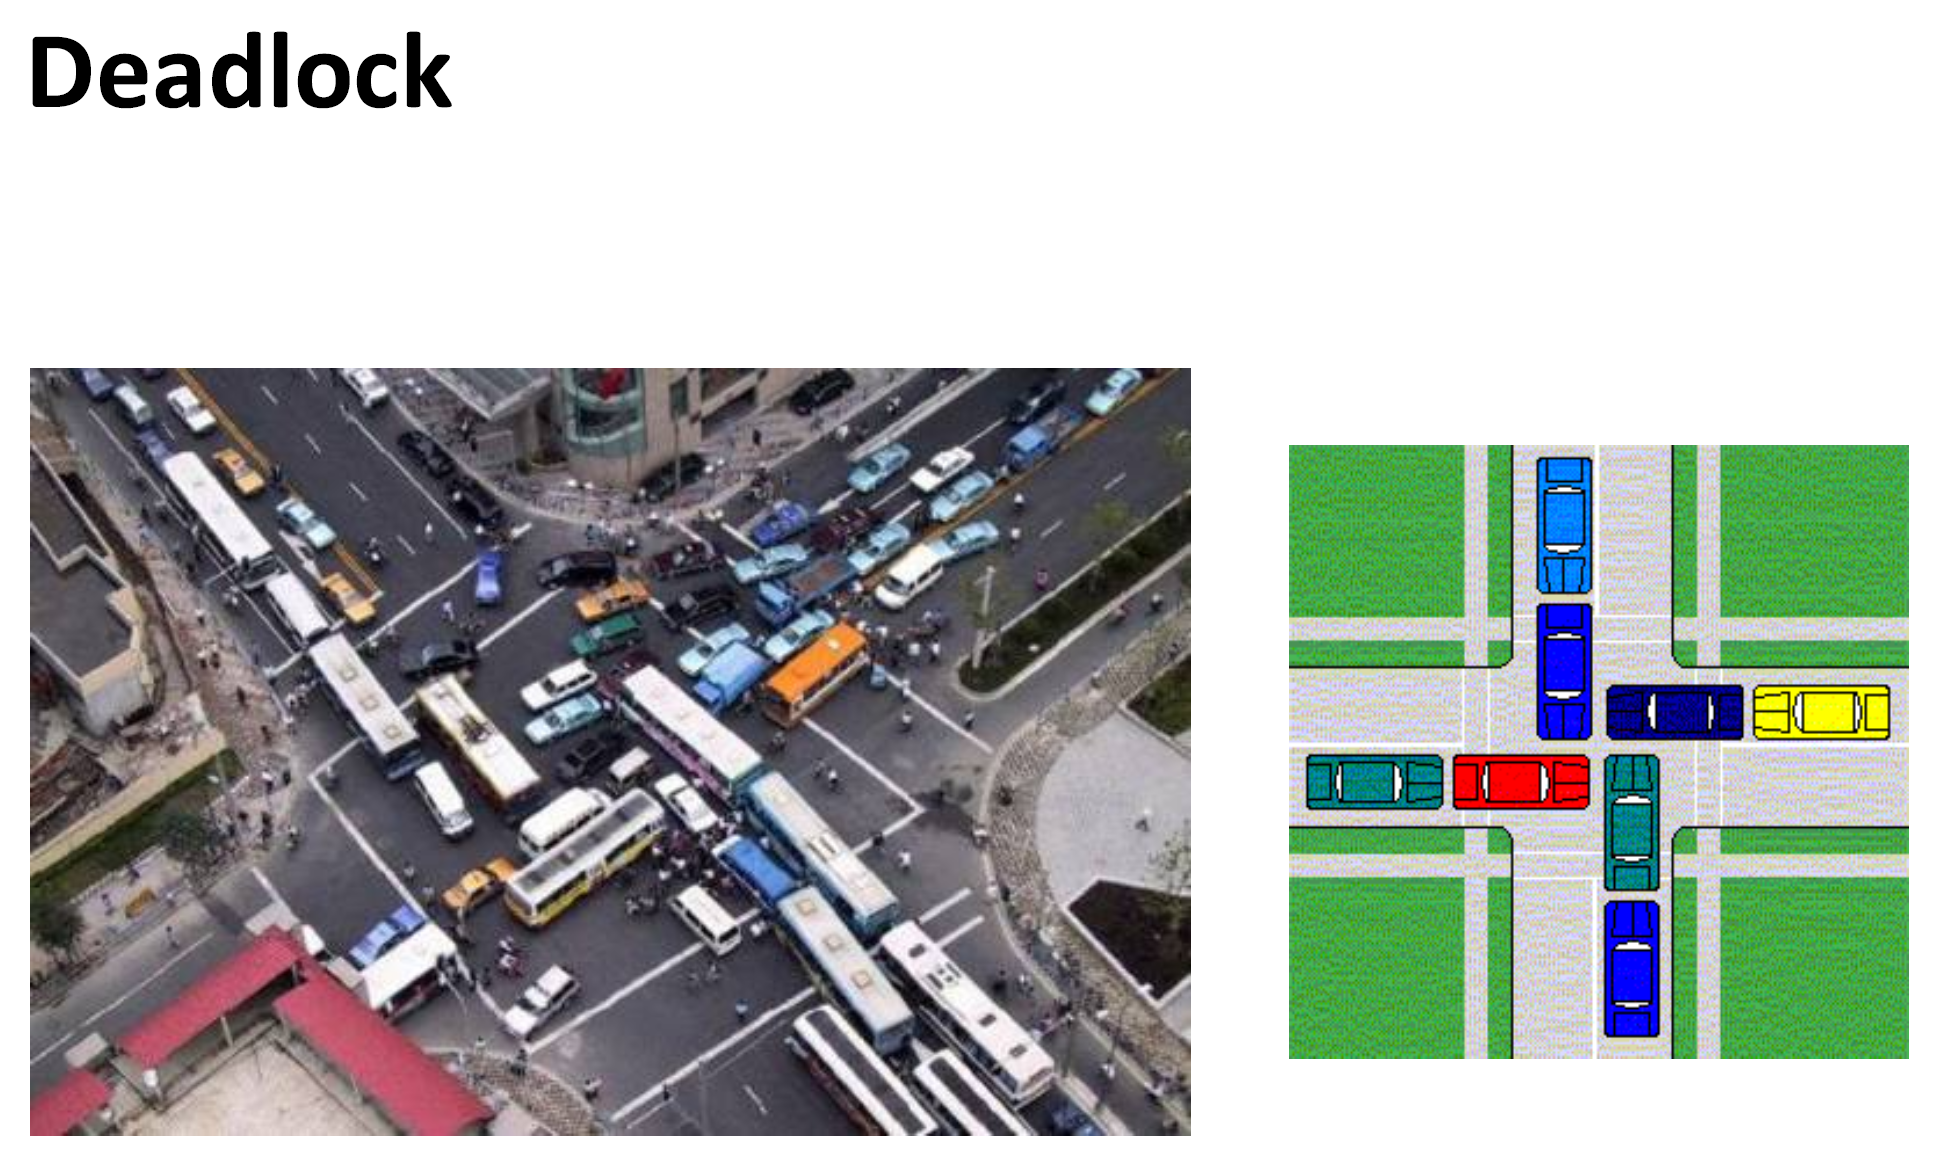
\includegraphics[width=\textwidth]{figures/zlx3.png}
        \end{figure}
    
    \end{frame}

    \section{不要忘了总结}

    \section*{致谢}

    \begin{frame}
        \setbeamertemplate{background}{}
        \frametitle{致谢}
        \begin{columns}
            \begin{column}{.5\linewidth}
                祝大家期末顺利!
                
                谢谢聆听!
            \end{column}
            \begin{column}{.5\linewidth}
                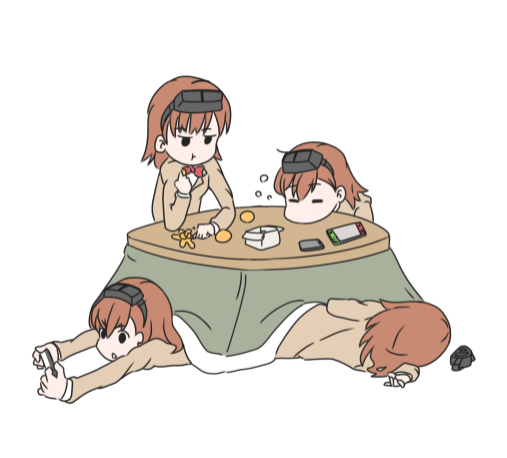
\includegraphics[width=.4\paperwidth]{figures/misaka558.png}
            \end{column}
        \end{columns}
    \end{frame}
    
\end{document}